\chapter{Development, Implementation, and Testing}
Model development is focused on obtaining a mathematical expression for modelling the two area power system and the PI controller, in addition to specifying the neural network architectures for experiments. Implementation primarily focuses on the DDPG training algorithm along with Python class implementations for the environment, PI controllers, and neural networks.

PROVIDE AND OVERVIEW OF THE SOFTWARE THAT HAS BEEN DEVELOPED - COMMUNICATE THIS IDEA BY CREATING A TREE LIKE STRUCTURE

\begin{figure}[h]
	\centering
	% Define block styles
\tikzstyle{script} = [draw, rectangle, fill=magenta!20, text width=8em, minimum height=2em, text centered, rounded corners, node distance=6cm]
\tikzstyle{class} = [draw, rectangle, fill=orange!20, text width=8em, minimum height=2em, text centered, rounded corners, node distance=2cm]
\tikzstyle{subclass} = [draw, rectangle, fill=yellow!20, text width=8em, minimum height=2em, text centered, rounded corners, node distance=2.5cm]

\newcommand*\circled[1]{\tikz[baseline=(char.base)]{
            \node[shape=circle,draw,inner sep=2pt] (char) {#1};}}

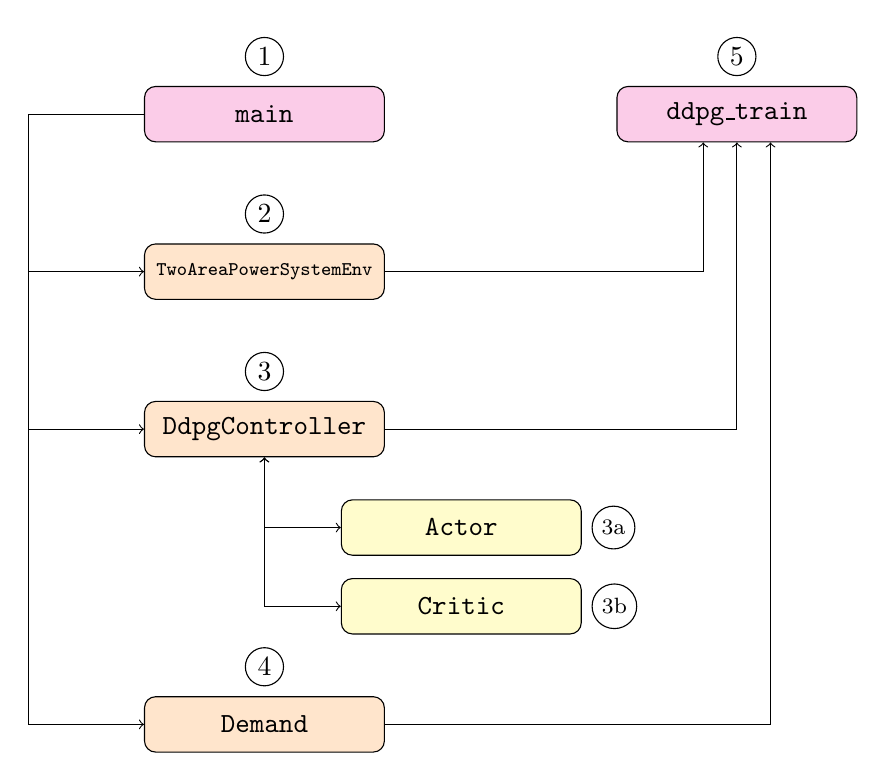
\begin{tikzpicture}[node distance = 2cm, auto]
    
    % Place script nodes
    \node [script, label=\circled{1}] (main) {\texttt{main}};
    \node [coordinate, left of=main, node distance=3cm] (p1) {};
    \node [script, right of=main, label=\circled{5}] (ddpg) {\texttt{ddpg\_train}};
  	
  	% Place class nodes
    \node [class, below of=main, label=\circled{2}] (env) {\scriptsize \texttt{TwoAreaPowerSystemEnv}};
    \node [class, below of=env, label=\circled{3}] (agent) {\texttt{DdpgController}};
    \node [coordinate, right of=agent, node distance=2.5cm] (p2) {};
    \node [class, below of=agent, node distance=3.75cm, label=\circled{4}] (demand) {\texttt{Demand}};
    
    % Place subclass node
    \node [subclass, below of=p2, node distance=1.25cm, label=0:\circled{\footnotesize 3a}] (actor) {\texttt{Actor}};
    \node [subclass, below of=actor, node distance=1cm, label=0:\circled{\footnotesize 3b}] (critic) {\texttt{Critic}};
    
    % Draw edges to classes
    \draw (main) -- (p1);
    \draw [->] (p1) |- (env);
    \draw [->] (p1) |- (agent);
    \draw [->] (p1) |- (demand);
    
    % Draw edge to subclass
    \draw[<->] (agent) |- (actor);
    \draw[<->] (agent) |- (critic);
    
    % Draw edge to training function
    \draw [->] (env) -| (ddpg.220);
    \draw [->] (agent) -| (ddpg);
    \draw [->] (demand) -| (ddpg.320);
    
\end{tikzpicture}
	\caption{text}
\end{figure}

%---------------- S: Environment

\section{Environment Model} \label{ssec:env_modelling}
The two area power system model described in \textsection \ref{ssec:modelling_two_area_system}, and shown in Figure \ref{fig:208_two_area_pi_control_model}, was converted from the frequency domain to the temporal domain. This provides the reinforcement learning architectures, outlined in \textsection \ref{sec:reinforcement_learning}, with the ability to export control signals to the power system at each time step. This approach is common practice when developing environments for reinforcement learning \cite{Brockman2016}. Additionally, frequency domain simulation techniques, such as Laplacian transforms, have strict initial condition assumptions \cite{Ogat2010}, which limit the application of this technology in real world applications.

Higher order ordinary differential equations and systems involving higher order ordinary differential equations provide a more compact system representation; however, to accommodate numerical analysis schemes, such as Runge-Kutta, the environment system was expressed as a system of first-order linear ordinary differential equations.

\begin{figure}[h]
	\centering
	\resizebox{\textwidth}{!}{%----------- Create a fancy summing block
\tikzset{add/.style n args={4}{
		minimum width=6mm,
		path picture={
			\draw[black] 
			(path picture bounding box.south east) -- (path picture bounding box.north west)
			(path picture bounding box.south west) -- (path picture bounding box.north east);
			\node at ($(path picture bounding box.south)+(0,0.13)$)     {\tiny #1};
			\node at ($(path picture bounding box.west)+(0.13,0)$)      {\tiny #2};
			\node at ($(path picture bounding box.north)+(0,-0.13)$)    {\tiny #3};
			\node at ($(path picture bounding box.east)+(-0.13,0)$)     {\tiny #4};
		}
	}
}

%----------- Block style 1
\tikzstyle{block1} = [draw, fill=white!80!green, rectangle, 
minimum height=3em, minimum width=6em, node distance=2.5cm]

%----------- Block style 2
\tikzstyle{block2} = [draw, fill=white!80!green, rectangle, 
minimum height=3em, minimum width=3em, node distance=2.5cm]

%----------- Sum style
\tikzstyle{sum} = [draw, fill=white!80!green, circle, node distance=2cm]

%----------- Input style
\tikzstyle{input} = [coordinate, node distance=4cm]

%----------- Output style
\tikzstyle{output} = [coordinate, node distance=4cm]

%----------- Pin style
\tikzstyle{pinstyle} = [pin edge={to-,thin,black}]


\begin{tikzpicture}	
	% Tie line nodes
	\node [sum, add={$-$}{}{+}{ }] (sum1) {};
	\node [block1, right of=sum1, label=above:{Tie Line}] (tieline) {$\frac{2\pi T_{12}}{s}$};
	\node [output, right of=tieline, node distance=3cm] (out) {};
	\node [coordinate, above of=out, node distance=5cm] (c1) {};
	\node [coordinate, below of=out, node distance=5cm] (c2) {};
	\node [block2, left of=c2] (a12) {$-a_{12}$};
	
	% Position a reference coordinate for drawing
	\node [coordinate, left of=sum1, node distance=2.5cm] (c3) {};
	\node [coordinate, above of=c3, node distance=0.75cm] (c4) {};
	\node [coordinate, below of=c3, node distance=0.75cm] (c5) {};
	
	% Create nodes for upper leg
	\node [block1, above of=c3, node distance=3.5cm, label=above:{Gen. Load 1}] (genload1) {$\frac{K_{gl1}}{T_{gl1}s+1}$};
	\node [coordinate, right of=genload1, node distance=1.5cm] (c6) {};
	\node [sum, left of=genload1, add={$-$}{+}{$-$}{}, node distance=2.5cm] (sum2) {};
	\node [coordinate, below of=sum2] (p11) {};
	\node [coordinate, left of=p11, node distance=0.5cm, label=left:{$\Delta P_{L1}(s)$}] (p12) {};
	\node [block1, left of=sum2, node distance=3.5cm, label=above:{Turbine 1}] (turbine1) {$\frac{K_{t1}}{T_{t1}s+1}$};
	\node [block1, left of=turbine1, node distance=4.5cm, label=above:{Governor 1}] (governor1) {$\frac{K_{g1}}{T_{g1}s+1}$};
	\node [coordinate, left of=governor1, node distance=3cm] (c8) {};
	\node [coordinate, left of=c5, node distance=13.5cm] (c10) {};
	\node [coordinate, left of=c1, node distance=21.5cm] (c12) {};
	
	
	
	% Create nodes for lower leg
	\node [block1, below of=c3, node distance=3.5cm, label=above:{Gen. Load 2}] (genload2) {$\frac{K_{gl1}}{T_{gl1}s+1}$};
	\node [coordinate, right of=genload2, node distance=1.5cm] (c7) {};
	\node [sum, left of=genload2, add={$-$}{+}{$-$}{}, node distance=2.5cm] (sum3) {};
	\node [coordinate, above of=sum3] (p21) {};
	\node [coordinate, left of=p21, node distance=0.5cm, label=left:{$\Delta P_{L2}(s)$}] (p22) {};
	\node [block1, left of=sum3, node distance=3.5cm, label=above:{Turbine 2}] (turbine2) {$\frac{K_{t2}}{T_{t2}s+1}$};
	\node [block1, left of=turbine2, node distance=4.5cm, label=above:{Governor 2}] (governor2) {$\frac{K_{g2}}{T_{g2}s+1}$};
	\node [coordinate, left of=governor2, node distance=3cm] (c9) {};
	\node [coordinate, left of=c4, node distance=13.5cm] (c11) {};
	\node [coordinate, left of=a12, node distance=19cm] (c13) {};
	
	
	% Connect the tieline nodes
	\draw [->] (sum1) -- (tieline);
	\draw (tieline) -- node [label=below:{$x_5(t)$}] {} (out);
	
	% Connect nodes in upper block
	\draw (out) -- (c1);
	\draw [->] (c1) -| (sum2);
	
	\draw [->] (governor1) -- node [label=above:{$x_2(t)$}] {} (turbine1);
	\draw [->] (turbine1) -- node [label=above:{$x_3(t)$}] {} (sum2);
	\draw [->] (sum2) -- (genload1);
	\draw [->] (genload1) -| node [label=above:{$x_4(t)$}] {} (sum1);
	\draw (c6) |- (c4);
	\draw [->] (c8) -- node [label=above:{$u_1(t)$}] {} (governor1);
	\draw (p12) -- (p11);
	\draw [->] (p11) -- (sum2);
	\draw [->] (c4) -- (c11);
	\draw [->] (c1) -- (c12);
	
	
	% Connect nodes in lower block
	\draw (out) -- (c2);
	\draw [->] (c2) -- (a12);
	\draw [->] (a12) -| (sum3);
	\draw [->] (governor2) -- node [label=below:{$x_7(t)$}] {} (turbine2);
	\draw [->] (turbine2) -- node [label=below:{$x_8(t)$}] {} (sum3);
	\draw [->] (sum3) -- (genload2);
	\draw [->] (genload2) -| node [label=below:{$x_9(t)$}] {} (sum1);
	\draw (c7) |- (c5);
	\draw [->] (c9) -- node [label=below:{$u_2(t)$}] {} (governor2);
	\draw (p22) -- (p21);
	\draw [->] (p21) -- (sum3);
	\draw [->] (c5) -- (c10);
	\draw [->] (a12) -- (c13);
	
\end{tikzpicture}}
	\caption[Two-area power system ODE derivation]{Variable assignment for a two area power system environment to model in the temporal domain}
	\label{4101_two_area_power_system_temporal_model}
\end{figure}

Suppose variables are assigned to the power system according to Figure \ref{4101_two_area_power_system_temporal_model}. The first order system of linear ordinary differential equations for area 1 is:
\begin{align}
	\dot{x}_2(t) &= \frac{1}{T_{sg_1}}\big( K_{sg_1} u_1(t) - x_2(t) \big) \label{eq:4101} \\
	\dot{x}_3(t) &= \frac{1}{T_{t_1}} \big( K_{t_1} x_2(t) - x_3(t) \big) \label{eq:4102} \\
	\dot{x}_4(t) &= \frac{1}{T_{gl_1}} \bigg( K_{gl_1} \big( x_3(t) - x_5(t) - \Delta p_{L1}(t) \big) - x_4(t) \bigg) \label{eq:4103}  \\
	\dot{x}_5(t) &= 2 \pi T_{12} \big( x_4(t) - x_9(t) \big) \label{eq:4104} \\
	\dot{x}_7(t) &= \frac{1}{T_{sg_2}}\big( K_{sg_2} u_2(t) - x_7(t) \big) \label{eq:4105} \\
	\dot{x}_8(t) &= \frac{1}{T_{t_2}} \big( K_{t_2} x_7(t) - x_8(t) \big) \label{eq:4106} \\
	\dot{x}_9(t) &= \frac{1}{T_{gl_2}} \bigg( K_{gl_2} \big( x_8(t) - x_5(t) - \Delta p_{L2}(t) \big) - x_9(t) \bigg) \label{eq:4107}
\end{align}

A full derivation of the first order linear system described by Equations \ref{eq:4101} to \ref{eq:4107} is described in Appendix \ref{app:C1_power_system_ode}. The equations were implemented as a method \verb|int_power_system_sim| in a Python class \verb|TwoAreaPowerSystemEnv|. Implementation for \verb|int_power_system_sim| is detailed in Appendix \ref{app:implementation_of_power_system_model}.

%---------------- S: PI Controller

\section{Classical PI Controller Model}
The proportional integral (PI) controller was converted from the frequency domain to the temporal domain, as outlined in the approach from \textsection \ref{ssec:environment_and_pi}.

\begin{figure}[h]
	\begin{minipage}[b]{0.5\textwidth}
		\resizebox{7.0cm}{!}{%----------- Create a fancy summing block
\tikzset{add/.style n args={4}{
		minimum width=6mm,
		path picture={
			\draw[black] 
			(path picture bounding box.south east) -- (path picture bounding box.north west)
			(path picture bounding box.south west) -- (path picture bounding box.north east);
			\node at ($(path picture bounding box.south)+(0,0.13)$)     {\tiny #1};
			\node at ($(path picture bounding box.west)+(0.13,0)$)      {\tiny #2};
			\node at ($(path picture bounding box.north)+(0,-0.13)$)    {\tiny #3};
			\node at ($(path picture bounding box.east)+(-0.13,0)$)     {\tiny #4};
		}
	}
}

%----------- Block style 1
\tikzstyle{block1} = [draw, fill=white!80!green, rectangle, 
minimum height=3em, minimum width=6em, node distance=2.5cm]

%----------- Block style 2
\tikzstyle{block2} = [draw, fill=white!80!blue, rectangle, 
minimum height=3em, minimum width=3em, node distance=2.5cm]

%----------- Sum style
\tikzstyle{sum} = [draw, fill=white!80!blue, circle, node distance=2cm]

%----------- Input style
\tikzstyle{input} = [coordinate, node distance=4cm]

%----------- Output style
\tikzstyle{output} = [coordinate, node distance=4cm]

%----------- Pin style
\tikzstyle{pinstyle} = [pin edge={to-,thin,black}]

\begin{tikzpicture}	
	% Initial position node
	\node [coordinate] (c1) {};
	
	
	% Create nodes for upper leg
	\node [sum, above of=c1, add={$-$}{}{+}{}, node distance=3.5cm] (sum4) {};
	\node [coordinate, above of=sum4, node distance=1.25cm] (c10) {};
	\node [coordinate, right of=c10, node distance=2cm] (c12) {};
	\node [coordinate, right of=sum4, node distance=2cm] (c2) {};
	\node [coordinate, above of=c2] (c4) {};
	\node [block2, below of=sum4, node distance=1.75cm] (r1) {$R_1$};
	\node [coordinate, below of=r1] (c6) {};
	\node [coordinate, right of=c6, node distance=2cm] (c8) {};
	\node [block2, left of=sum4] (int1) {$\frac{K_{i_1}}{s}$};
	\node [sum, left of=int1, add={+}{ }{+}{ }] (sum6) {};
	\node [block2, below of=sum6, node distance=1.75cm] (b1) {$b_1$};
	
	
	% Connect nodes
	\draw [->] (sum4) -- node [at end, label=right:{$u_1(t)$}] {} (c2);
	\draw [->] (r1) -- (sum4);
	\draw [->] (b1) -- (sum6);
	\draw [->] (sum6) -- (int1);
	\draw [->] (int1) -- node [label=above:{$x_1(t)$}] {} (sum4);
	\draw [->] (c8) -| node [at start, label=right:{$x_4(t)$}] {} (r1);
	\draw [->] (c8) -| (b1);
	\draw [->] (c12) -| node [at start, label=right:{$x_5(t)$}] {} (sum4);
	\draw [->] (c12) -| (sum6);
	
\end{tikzpicture}}
		\caption[Area 1 PI controller ODE derivation]{Variable assignment for the PI controller for area 1 in order to model in the temporal domain}
		\label{fig:4102_two_area_pi_controller_temporal_1}
	\end{minipage}
	\hspace{0.1cm}
	\begin{minipage}[b]{0.5\textwidth}
		\resizebox{7.2cm}{!}{%----------- Create a fancy summing block
\tikzset{add/.style n args={4}{
		minimum width=6mm,
		path picture={
			\draw[black] 
			(path picture bounding box.south east) -- (path picture bounding box.north west)
			(path picture bounding box.south west) -- (path picture bounding box.north east);
			\node at ($(path picture bounding box.south)+(0,0.13)$)     {\tiny #1};
			\node at ($(path picture bounding box.west)+(0.13,0)$)      {\tiny #2};
			\node at ($(path picture bounding box.north)+(0,-0.13)$)    {\tiny #3};
			\node at ($(path picture bounding box.east)+(-0.13,0)$)     {\tiny #4};
		}
	}
}

%----------- Block style 1
\tikzstyle{block1} = [draw, fill=white!80!blue, rectangle, 
minimum height=3em, minimum width=6em, node distance=2.5cm]

%----------- Block style 2
\tikzstyle{block2} = [draw, fill=white!80!blue, rectangle, 
minimum height=3em, minimum width=3em, node distance=2.5cm]

%----------- Sum style
\tikzstyle{sum} = [draw, fill=white!80!blue, circle, node distance=2cm]

%----------- Input style
\tikzstyle{input} = [coordinate, node distance=4cm]

%----------- Output style
\tikzstyle{output} = [coordinate, node distance=4cm]

%----------- Pin style
\tikzstyle{pinstyle} = [pin edge={to-,thin,black}]

\begin{tikzpicture}	
	% Initial position node
	\node [coordinate] (c1) {};
	
	
	% Create nodes for lower leg
	\node [sum, below of=c1, add={+}{}{$-$}{}, node distance=3.5cm] (sum5) {};
	\node [coordinate, below of=sum5, node distance=1.25cm] (c11) {};
	\node [coordinate, right of=c11, node distance=2cm] (c13) {};
	\node [coordinate, right of=sum5, node distance=2cm] (c3) {};
	\node [coordinate, above of=c3] (c5) {};
	\node [block2, above of=sum5, node distance=1.75cm] (r2) {$R_2$};
	\node [coordinate, above of=r2] (c7) {};
	\node [coordinate, right of=c7, node distance=2cm] (c9) {};
	\node [block2, left of=sum5] (int2) {$\frac{K_{i_2}}{s}$};
	\node [sum, left of=int2, add={+}{ }{+}{ }] (sum7) {};
	\node [block2, above of=sum7, node distance=1.75cm] (b2) {$b_2$};
	
	
	% Connect nodes
	\draw [->] (sum5) -- node [at end, label=right:{$u_2(t)$}] {} (c3);
	\draw [->] (r2) -- (sum5);
	\draw [->] (b2) -- (sum7);
	\draw [->] (sum7) -- (int2);
	\draw [->] (int2) -- node [label=below:{$x_6(t)$}] {} (sum5);
	\draw [->] (c9) -| node [at start, label=right:{$x_9(t)$}] {} (r2);
	\draw [->] (c9) -| (b2);
	\draw [->] (c13) -| node [at start, label=right:{$-x_5(t)$}] {} (sum5);
	\draw [->] (c13) -| (sum7);
	
\end{tikzpicture}}
		\caption[Area 2 PI controller ODE derivation]{Variable assignment for the PI controller for area 2 in order to model in the temporal domain}
		\label{fig:4103_two_area_pi_controller_temporal_2}
	\end{minipage}
\end{figure}

Suppose variables are assigned to the controller for area 1 and the controller for area 2 according to Figures \ref{fig:4102_two_area_pi_controller_temporal_1} and \ref{fig:4103_two_area_pi_controller_temporal_2}, respectively. The first order system of linear differential equations for the PI controller are:
\begin{align}
	\dot{x}_1(t) &= b_1 \Delta f_1(t) + x_5(t) \label{eq:4108} \\
	\dot{x}_6(t) &= b_2 \Delta f_2(t) - x_5(t) \label{eq:4109}
\end{align}

Note that once the PI controller has stepped forward in time during simulation the actual control signals exported from the controller are $u_1(t)$ and $u_2(t)$. These are expressed as:
\begin{align}
	u_1(t) &= x_1(t) + x_5(t) - R_1 x_4(t) \\
	u_2(t) &= x_6(t) - x_5(t) - R_2 x_9(t) 
\end{align}

A full derivation of the first order linear system described by equations \ref{eq:4108} and \ref{eq:4109} is described in Appendix \ref{sec:temporal_domain_for_pi_controller}. The system of equations is implemented as a method \verb|int_control_system_sim| in a Python class \verb|ClassicalPiController|. Implementation for \verb|int_control_system_sim| is detailed in Appendix \ref{sec:implementation_of_controller}.

%---------------- S: Neural Network Controller

\section{DDPG Controller}
The DDPG algorithm was implemented using a Python class \verb|DdpgController|, and a function called \verb|ddpg_train|.

When an instance of the \verb|DdpgController| class is created a number of critical tasks are performed. These include initialisation of neural networks in memory for the actor and critic, and their associated target networks, declaration of DDPG hyperparameters discussed in \textsection \ref{ssec:deep_deterministic_policy_gradient}, initialisation of a replay buffer for storing agent experience, and the initialisation of an Ornstein–Uhlenbeck process to add exploratory noise to action signals. Additionally, the \verb|DdpgController| class defines methods used for model training. A description of key methods is provided in Table \ref{tab:4103}. The \verb|DdpgController| class implementation can be found in Appendix \ref{app:implementation_ddpg_controller}.

\begin{table}[h]
	\centering
	\cprotect\caption{Description of key methods for the \verb|DdpgController| class}
	\begin{tabular}{lp{12cm}}
		\toprule
		\textbf{Method} & \textbf{Description} \\
		\midrule
		\verb|step| & Stores the current experience tuple, $(s_t, a_t, r_t, S_{t+1})$, in the experience replay buffer, and calls the method \verb|learn|\\
		 & \\
		\verb|act| & Takes a state as input and uses this for a call to the neural network method \verb|forward| which returns an action\\
		 & \\
		\verb|learn| & Performs gradient descent, using backpropagation, on the actor and critic loss functions to adjust weights for each respective network using a set of random uniformly sampled experiences from the experience replay buffer\\
		\bottomrule
	\end{tabular}\label{tab:4103}
\end{table}

%---------------- S: DDPG Algorithm

\section{DDPG Training Algorithm}
Actor and critic neural networks are trained using the DDPG algorithm shown in listing \ref{ssec:deep_deterministic_policy_gradient}. 

The function \verb|ddpg_train| takes environment and agent class instances as inputs. The function runs training for a specified number of episodes. For each episode, \verb|ddpg_train| takes time steps of 0.01 sec until the episode triggers a termination condition. During each time step, \verb|ddpg_train| will obtain an action from the agent given the current state, obtain the power demand signal for the given time step, and step the environment forward using the agent's action and power demanded. The function the makes a call to the agent method \verb|step|, which stores the experience in the replay buffer and trains the neural network.